\documentclass{standalone}
\usepackage{tikz}
\usetikzlibrary{patterns, positioning}

\begin{document}
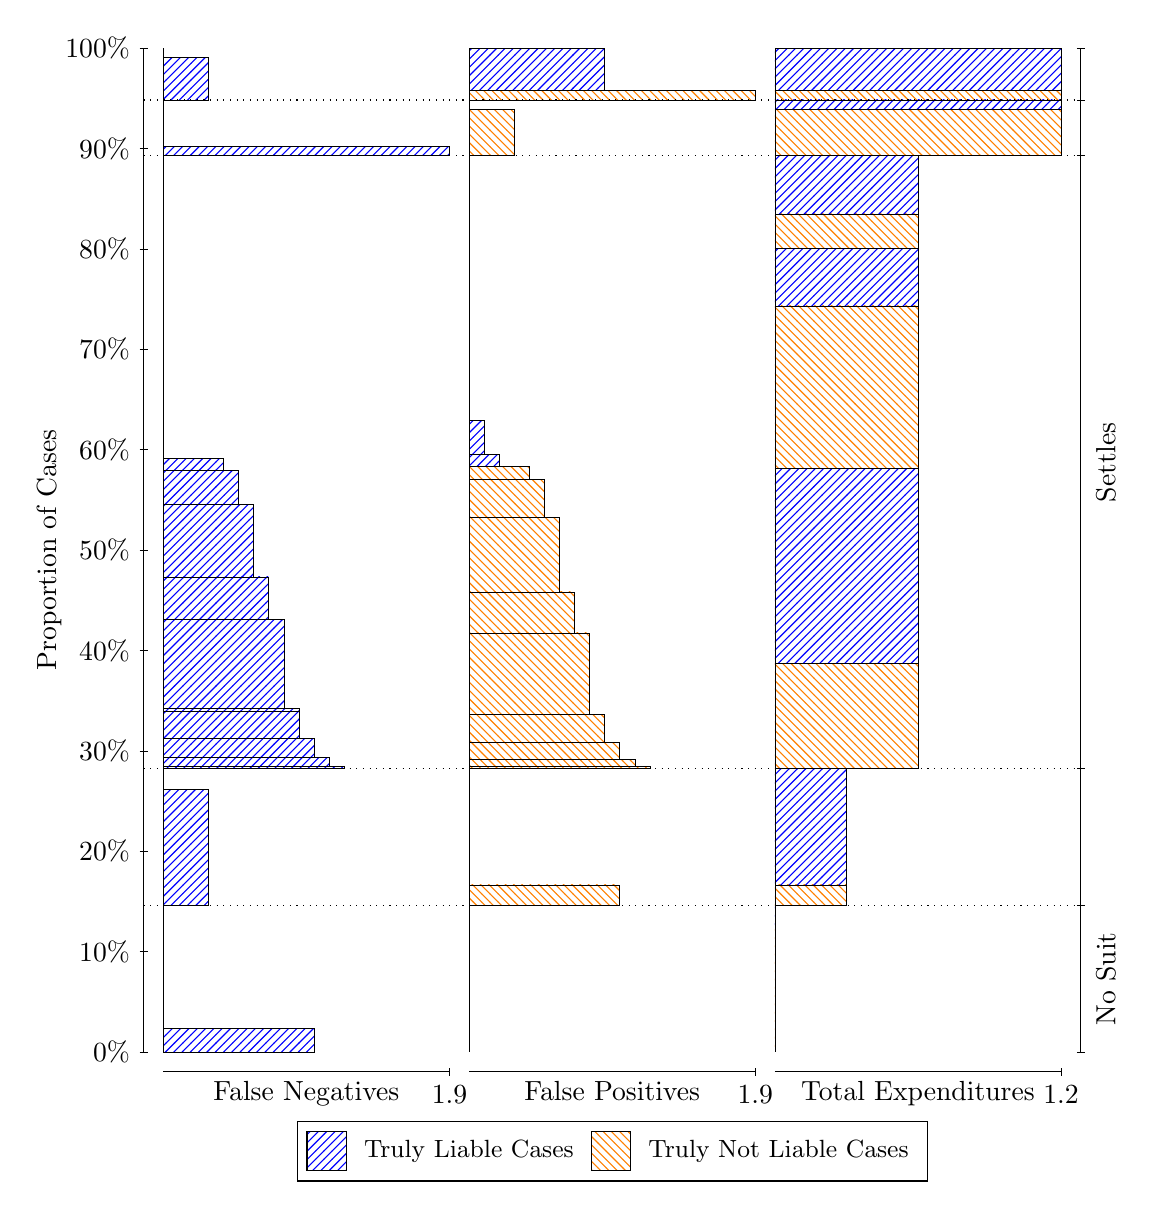
\begin{tikzpicture}
\draw[black, very thin] (1.5,1.75) -- (1.5,14.5);
\node[rotate=90, anchor=center] at (0.3, 8.125) {Proportion of Cases};
\draw[black, very thin] (1.45,1.75) -- (1.55,1.75);
\node[anchor=east] at (1.45, 1.75) {0\%};
\draw[black, very thin] (1.45,3.025) -- (1.55,3.025);
\node[anchor=east] at (1.45, 3.025) {10\%};
\draw[black, very thin] (1.45,4.3) -- (1.55,4.3);
\node[anchor=east] at (1.45, 4.3) {20\%};
\draw[black, very thin] (1.45,5.575) -- (1.55,5.575);
\node[anchor=east] at (1.45, 5.575) {30\%};
\draw[black, very thin] (1.45,6.85) -- (1.55,6.85);
\node[anchor=east] at (1.45, 6.85) {40\%};
\draw[black, very thin] (1.45,8.125) -- (1.55,8.125);
\node[anchor=east] at (1.45, 8.125) {50\%};
\draw[black, very thin] (1.45,9.4) -- (1.55,9.4);
\node[anchor=east] at (1.45, 9.4) {60\%};
\draw[black, very thin] (1.45,10.675) -- (1.55,10.675);
\node[anchor=east] at (1.45, 10.675) {70\%};
\draw[black, very thin] (1.45,11.95) -- (1.55,11.95);
\node[anchor=east] at (1.45, 11.95) {80\%};
\draw[black, very thin] (1.45,13.225) -- (1.55,13.225);
\node[anchor=east] at (1.45, 13.225) {90\%};
\draw[black, very thin] (1.45,14.5) -- (1.55,14.5);
\node[anchor=east] at (1.45, 14.5) {100\%};

\draw[black, very thin] (13.4,1.75) -- (13.4,14.5);
\draw[black, very thin] (13.35,1.75) -- (13.45,1.75);
\node[anchor=west] at (13.35, 1.75) {};
\draw[black, very thin] (13.35,3.6073) -- (13.45,3.6073);
\node[anchor=west] at (13.35, 3.6073) {};
\draw[black, very thin] (13.35,5.3472) -- (13.45,5.3472);
\node[anchor=west] at (13.35, 5.3472) {};
\draw[black, very thin] (13.35,13.132) -- (13.45,13.132);
\node[anchor=west] at (13.35, 13.132) {};
\draw[black, very thin] (13.35,13.84) -- (13.45,13.84);
\node[anchor=west] at (13.35, 13.84) {};
\draw[black, very thin] (13.35,14.5) -- (13.45,14.5);
\node[anchor=west] at (13.35, 14.5) {};

\draw[black, very thin, pattern color=blue, pattern=north east lines] (1.75,1.75) rectangle (3.6623,2.0483);
\draw[black, very thin, pattern color=orange, pattern=north west lines] (1.75,2.0483) rectangle (1.75,3.6073);
\draw[black, very thin, pattern color=blue, pattern=north east lines] (1.75,3.6073) rectangle (2.3237,5.0837);
\draw[black, very thin, pattern color=orange, pattern=north west lines] (1.75,5.0837) rectangle (1.75,5.3472);
\draw[black, very thin, pattern color=blue, pattern=north east lines] (1.75,5.3472) rectangle (4.0447,5.3774);
\draw[black, very thin, pattern color=blue, pattern=north east lines] (1.75,5.3774) rectangle (3.8535,5.4896);
\draw[black, very thin, pattern color=blue, pattern=north east lines] (1.75,5.4896) rectangle (3.6623,5.7286);
\draw[black, very thin, pattern color=blue, pattern=north east lines] (1.75,5.7286) rectangle (3.4711,6.0748);
\draw[black, very thin, pattern color=blue, pattern=north east lines] (1.75,6.0748) rectangle (3.4711,6.1182);
\draw[black, very thin, pattern color=blue, pattern=north east lines] (1.75,6.1182) rectangle (3.2798,7.2389);
\draw[black, very thin, pattern color=blue, pattern=north east lines] (1.75,7.2389) rectangle (3.0886,7.7837);
\draw[black, very thin, pattern color=blue, pattern=north east lines] (1.75,7.7837) rectangle (2.8974,8.7077);
\draw[black, very thin, pattern color=blue, pattern=north east lines] (1.75,8.7077) rectangle (2.7061,9.1385);
\draw[black, very thin, pattern color=blue, pattern=north east lines] (1.75,9.1385) rectangle (2.5149,9.2875);
\draw[black, very thin, pattern color=orange, pattern=north west lines] (1.75,9.2875) rectangle (1.75,13.132);
\draw[black, very thin, pattern color=blue, pattern=north east lines] (1.75,13.132) rectangle (5.3833,13.25);
\draw[black, very thin, pattern color=orange, pattern=north west lines] (1.75,13.25) rectangle (1.75,13.84);
\draw[black, very thin, pattern color=blue, pattern=north east lines] (1.75,13.84) rectangle (2.3237,14.382);
\draw[black, very thin, pattern color=orange, pattern=north west lines] (1.75,14.382) rectangle (1.75,14.5);
\draw[black, very thin, pattern color=orange, pattern=north west lines] (5.6333,1.75) rectangle (5.6333,3.3091);
\draw[black, very thin, pattern color=blue, pattern=north east lines] (5.6333,3.3091) rectangle (5.6333,3.6073);
\draw[black, very thin, pattern color=orange, pattern=north west lines] (5.6333,3.6073) rectangle (7.5456,3.8708);
\draw[black, very thin, pattern color=blue, pattern=north east lines] (5.6333,3.8708) rectangle (5.6333,5.3472);
\draw[black, very thin, pattern color=orange, pattern=north west lines] (5.6333,5.3472) rectangle (7.9281,5.3732);
\draw[black, very thin, pattern color=orange, pattern=north west lines] (5.6333,5.3732) rectangle (7.7368,5.4654);
\draw[black, very thin, pattern color=orange, pattern=north west lines] (5.6333,5.4654) rectangle (7.5456,5.6808);
\draw[black, very thin, pattern color=orange, pattern=north west lines] (5.6333,5.6808) rectangle (7.3544,6.0389);
\draw[black, very thin, pattern color=orange, pattern=north west lines] (5.6333,6.0389) rectangle (7.1632,7.0734);
\draw[black, very thin, pattern color=orange, pattern=north west lines] (5.6333,7.0734) rectangle (6.9719,7.5928);
\draw[black, very thin, pattern color=orange, pattern=north west lines] (5.6333,7.5928) rectangle (6.7807,8.5379);
\draw[black, very thin, pattern color=orange, pattern=north west lines] (5.6333,8.5379) rectangle (6.5895,9.0183);
\draw[black, very thin, pattern color=orange, pattern=north west lines] (5.6333,9.0183) rectangle (6.3982,9.1913);
\draw[black, very thin, pattern color=blue, pattern=north east lines] (5.6333,9.1913) rectangle (6.0158,9.3403);
\draw[black, very thin, pattern color=blue, pattern=north east lines] (5.6333,9.3403) rectangle (5.8246,9.7711);
\draw[black, very thin, pattern color=blue, pattern=north east lines] (5.6333,9.7711) rectangle (5.6333,13.132);
\draw[black, very thin, pattern color=orange, pattern=north west lines] (5.6333,13.132) rectangle (6.207,13.722);
\draw[black, very thin, pattern color=blue, pattern=north east lines] (5.6333,13.722) rectangle (5.6333,13.84);
\draw[black, very thin, pattern color=orange, pattern=north west lines] (5.6333,13.84) rectangle (9.2667,13.959);
\draw[black, very thin, pattern color=blue, pattern=north east lines] (5.6333,13.959) rectangle (7.3544,14.5);
\draw[black, very thin, pattern color=orange, pattern=north west lines] (9.5167,1.75) rectangle (9.5167,3.3091);
\draw[black, very thin, pattern color=blue, pattern=north east lines] (9.5167,3.3091) rectangle (9.5167,3.6073);
\draw[black, very thin, pattern color=orange, pattern=north west lines] (9.5167,3.6073) rectangle (10.425,3.8708);
\draw[black, very thin, pattern color=blue, pattern=north east lines] (9.5167,3.8708) rectangle (10.425,5.3472);
\draw[black, very thin, pattern color=orange, pattern=north west lines] (9.5167,5.3472) rectangle (11.333,6.6892);
\draw[black, very thin, pattern color=blue, pattern=north east lines] (9.5167,6.6892) rectangle (11.333,9.1647);
\draw[black, very thin, pattern color=orange, pattern=north west lines] (9.5167,9.1647) rectangle (11.333,11.226);
\draw[black, very thin, pattern color=blue, pattern=north east lines] (9.5167,11.226) rectangle (11.333,11.953);
\draw[black, very thin, pattern color=orange, pattern=north west lines] (9.5167,11.953) rectangle (11.333,12.394);
\draw[black, very thin, pattern color=blue, pattern=north east lines] (9.5167,12.394) rectangle (11.333,13.132);
\draw[black, very thin, pattern color=orange, pattern=north west lines] (9.5167,13.132) rectangle (13.15,13.722);
\draw[black, very thin, pattern color=blue, pattern=north east lines] (9.5167,13.722) rectangle (13.15,13.84);
\draw[black, very thin, pattern color=orange, pattern=north west lines] (9.5167,13.84) rectangle (13.15,13.959);
\draw[black, very thin, pattern color=blue, pattern=north east lines] (9.5167,13.959) rectangle (13.15,14.5);
\draw[black, dotted] (1.5,3.6073) -- (13.4,3.6073);
\draw[black, dotted] (1.5,5.3472) -- (13.4,5.3472);
\draw[black, dotted] (1.5,13.132) -- (13.4,13.132);
\draw[black, dotted] (1.5,13.84) -- (13.4,13.84);
\draw[black, very thin] (1.75,1.5) -- (5.3833,1.5);
\node[anchor=north] at (3.5667, 1.5) {False Negatives};
\draw[black, very thin] (5.3833,1.45) -- (5.3833,1.55);
\node[anchor=north] at (5.3833, 1.45) {1.9};

\draw[black, very thin] (5.6333,1.5) -- (9.2667,1.5);
\node[anchor=north] at (7.45, 1.5) {False Positives};
\draw[black, very thin] (9.2667,1.45) -- (9.2667,1.55);
\node[anchor=north] at (9.2667, 1.45) {1.9};

\draw[black, very thin] (9.5167,1.5) -- (13.15,1.5);
\node[anchor=north] at (11.333, 1.5) {Total Expenditures};
\draw[black, very thin] (13.15,1.45) -- (13.15,1.55);
\node[anchor=north] at (13.15, 1.45) {1.2};

\node[black, centered, rotate=90] at (13.72, 2.6787) {No Suit};

\node[black, centered, rotate=90] at (13.72, 9.2394) {Settles};



\draw (7.449999999999999,1.5) node[draw=none] (baseCoordinate) {};
\begin{scope}[align=center]
        \matrix[scale=0.5, draw=black, below=0.5cm of baseCoordinate, nodes={draw}, column sep=0.1cm]{
            \node[rectangle, draw, minimum width=0.5cm, minimum height=0.5cm, pattern=north east lines, pattern color=blue] {}; &
            \node[draw=none, font=\small] (B) {Truly Liable Cases}; &
            \node[rectangle, draw, minimum width=0.5cm, minimum height=0.5cm, pattern=north west lines, pattern color=orange] {}; &
            \node[draw=none, font=\small] (B) {Truly Not Liable Cases}; \\
            };
\end{scope}

\end{tikzpicture}
\end{document}